\documentclass[11pt]{article}
\usepackage[margin=1.1in]{geometry}
\usepackage{mathptmx}
\usepackage{amsmath,amssymb}
\usepackage{graphicx}
\usepackage{booktabs}
\usepackage{caption}
\usepackage[colorlinks=true,linkcolor=black,citecolor=black,urlcolor=blue]{hyperref}
\usepackage{titlesec}
\usepackage{xcolor}

\captionsetup{font=small,labelfont=bf}
\titleformat{\section}{\large\bfseries}{\thesection}{0.7em}{}
\titleformat{\subsection}{\normalsize\bfseries}{\thesubsection}{0.7em}{}

\newcommand{\keyfinding}[1]{\vspace{2pt}\noindent\fbox{\parbox{0.97\linewidth}{#1}}\vspace{2pt}}

\title{\bf What Is Left of a Picture:\\[2pt]
\large Visual Content Is Written Into the Recurrent Memory of a Hybrid\\
Vision-Language Model, Then Discarded Unread}

\author{Vizuara Research}
\date{August 2026}

\begin{document}
\maketitle

\begin{abstract}
\noindent
In a transformer, an image persists: it becomes hundreds of key-value entries
that any later computation can attend to. In a hybrid linear-attention model it
does not. Most layers compress what they read into a fixed-size recurrent state
that later tokens overwrite. We ask what remains of an image in that state, and
whether the model uses it. Working with Zamba2-VL-7B, whose 81 decoder layers
all carry a Mamba2 mixer while only 13 additionally carry attention, we train
linear probes on the recurrent state alone and pair them with a causal channel
splice. Three findings. First, at the moment of writing the state is highly
informative about \emph{which} object is present ($83.1\%$ against a $12.5\%$
chance rate, $p = 6 \times 10^{-92}$) and only marginally informative about
\emph{how many} ($19.4\%$) or \emph{where} ($17.5\%$): it records gist, not
particulars. Second, this content collapses to chance within roughly 32 tokens
and never returns, while the model's own accuracy stays above $95\%$ out to 2048
tokens. Third, the splice explains the discrepancy: exchanging all 81 recurrent
states between two runs that saw different images leaves the answer unchanged
($17 \to 19$ of 30 following the model's own image), whereas exchanging the 13
attention caches flips it completely ($0$ of 30 own image, $15$ of 30 the
other), and exchanging both is indistinguishable from exchanging attention
alone. The recurrent memory therefore holds a real, measurable impression of the
image that plays no causal role in the answer. Every current mechanistic account
of visual hallucination is expressed in terms of attention over image tokens;
none of it can describe the six-sevenths of this model where no such attention
exists. Total compute: under \$30 of on-demand GPU rental.
\end{abstract}

\begin{figure}[h]
\centering
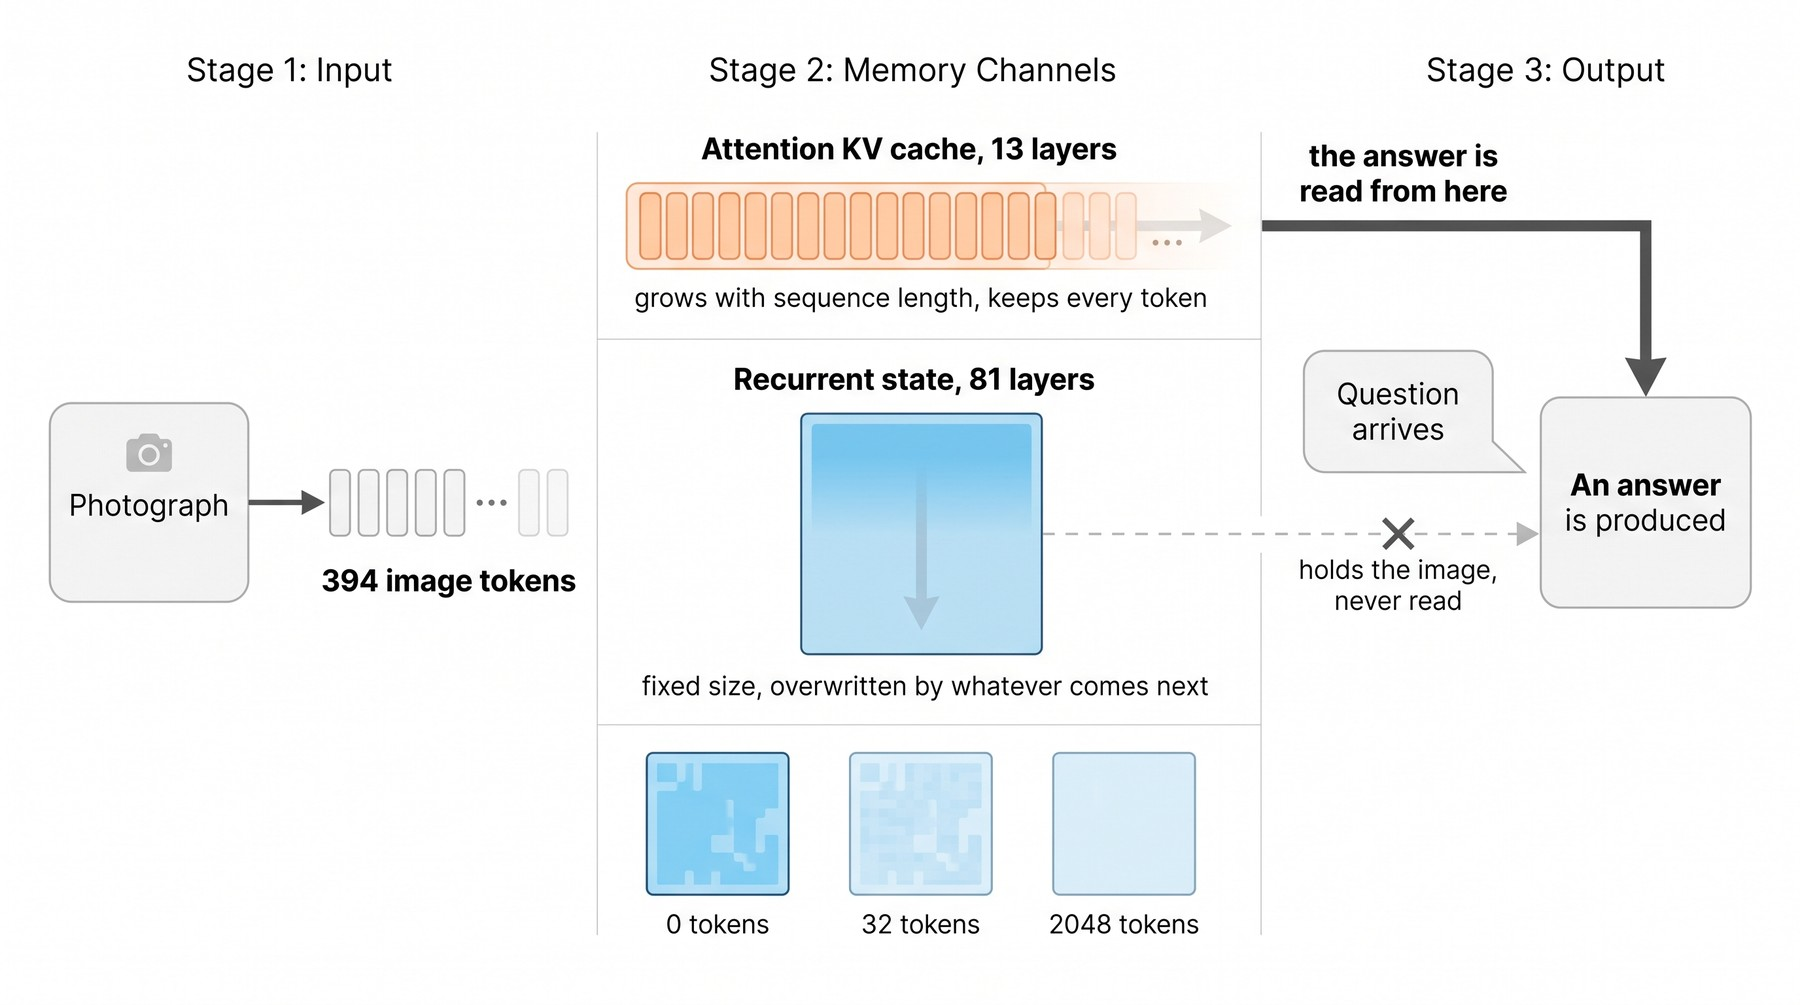
\includegraphics[width=0.98\linewidth]{../docs/assets/fig_idea.jpg}
\caption{\textbf{The idea.} A photograph becomes 394 image tokens and is written
into two memories at once: an attention KV cache that grows with the sequence,
present in 13 layers; and a fixed-size recurrent state that is overwritten by
whatever follows, present in all 81. The answer is read from the 13. The 81
hold the image and are never read.}
\end{figure}

\section{What Was Known Before, and What Is New Here}
\label{sec:novelty}

This section is placed before the results deliberately, so that every claim
below can be read against an explicit boundary.

\subsection*{What was already established}

\begin{itemize}\itemsep2pt
\item \textbf{Recurrent states in hybrid VLMs accumulate information, and
discarded tokens persist in them.} Jiang et al.~\cite{jiang2026stateful}
studied token reduction in hybrid Mamba-Transformer VLMs and introduced a
representation-based probing method measuring how much information from
discarded tokens is retained, concluding that reduction there behaves ``more
like compression than dropping.'' Their goal is prefill throughput.
\item \textbf{Vision-language models are sensitive to the order of image and
question, and the sensitivity has an attention-based explanation.}
Abhinandan et al.~\cite{abhinandan2026asktwice} identified a ``question-first
paradox'' across five open VLMs, traced it with logit-lens and a causal
attention knockout to a question ``stranded behind hundreds of image tokens,''
and resolved it by echoing the question on both sides of the image. Gupta and
Gandelsman~\cite{gupta2026modality} independently localised the same ordering
failure to a narrow mid-network region using activation patching.
\item \textbf{Visual attributes can be linearly recoverable from hidden states
yet unavailable to the model's own output.} Osaka et al.~\cite{osaka2026vab}
introduced a Visual Access Sweep over Qwen2.5-VL and InternVL3, defined a
Visual Access Boundary, and showed with a probe-versus-decode check that the
bottleneck sits at readout rather than at computation.
\end{itemize}

\subsection*{What none of that covers, and what we contribute}

\begin{table}[h]
\centering\small
\begin{tabular}{@{}p{0.44\linewidth}p{0.5\linewidth}@{}}
\toprule
\textbf{Prior work} & \textbf{Not addressed by it} \\
\midrule
Jiang et al.~\cite{jiang2026stateful}: probes retention of discarded tokens in
a hybrid VLM's recurrent state, for token reduction.
& Which \emph{visual properties} survive; how retention varies with distance
from the image; whether the retained content is causally used. \\[4pt]
Abhinandan et al.~\cite{abhinandan2026asktwice}; Gupta and
Gandelsman~\cite{gupta2026modality}: image/question ordering and its
attention-based mechanism.
& Both study attention-only VLMs (Qwen2.5-VL, InternVL3 and similar). Their
mechanism presupposes attention over image tokens and is undefined for a
recurrent layer. \\[4pt]
Osaka et al.~\cite{osaka2026vab}: probe-versus-decode gap in transformer VLMs.
& Transformer only. Does not ask whether a non-attentional memory carries
content, nor test it causally. \\
\bottomrule
\end{tabular}
\end{table}

\noindent Our contributions, none of which appear in the above:
\begin{enumerate}\itemsep1pt
\item The first property-resolved measurement of what an image becomes inside a
recurrent state: a gist-versus-particulars gradient at the moment of writing.
\item The first distance-resolved measurement of visual content in such a
state, showing collapse within about 32 tokens against flat behavioural
accuracy to 2048.
\item The first causal channel splice in a vision-language model that
exchanges the recurrent memory and the attention cache independently,
establishing that the recurrent contribution is not small but absent from the
causal path.
\item A demonstration that ``present but causally inert'' is a distinct state
from the availability/accessibility gap of~\cite{osaka2026vab}: there the
content is unreadable by the model; here it is unread.
\end{enumerate}

\section{Significance}
\label{sec:significance}

\keyfinding{\textbf{The short version.} A class of models now being deployed for
efficiency keeps most of its memory in a form that, for images, holds a real
impression that nothing ever reads. Every deployed mitigation for visual
hallucination targets the other one-seventh.}

\paragraph{For people building hybrid models.} The efficiency argument for
replacing attention layers with recurrent ones assumes the recurrent layers do
comparable work. For exact visual recall in this model they do none: the answer
survives the total destruction of all 81 recurrent states and does not survive
the replacement of 13 attention caches. That is a concrete design signal about
where the attention budget matters and where it can be cut, and it is
measurable with the instruments released here.

\paragraph{For people working on hallucination.} Contrastive decoding,
attention re-weighting and visual-attention diagnostics are all defined over
attention to image tokens. In a model that is six-sevenths recurrent, those
tools address a minority of the computation by construction. Our result is not
that the recurrent layers cause hallucination; it is that they have been
outside the reach of every method, and that they demonstrably contain
information which the current toolkit cannot see.

\paragraph{For interpretability more broadly.} The field's benchmarks and
agenda documents are written for dense transformers. This is a worked example
of a finding that only exists in a non-transformer architecture, obtained with
instruments that a transformer-only toolkit does not possess, and it argues
that architecture coverage is a real gap rather than a stylistic preference.

\paragraph{What a practitioner should do differently tomorrow.} If you evaluate
a hybrid VLM and want to know whether it saw something, do not probe its
recurrent state and conclude from a null that the information is absent, nor
from a positive that the model is using it. Neither inference is valid in this
architecture. Test the channel causally.

\section{Model and Instruments}

\paragraph{Model.} Zamba2-VL-7B~\cite{zamba2vl} pairs a Zamba2 hybrid language
backbone with a Qwen2.5-VL vision encoder. We verified its structure
empirically rather than from documentation: 81 decoder layers, \emph{all} of
which carry a Mamba2~\cite{dao2024mamba2} mixer, of which 13 (indices
$6, 11, 17, \dots, 77$) additionally carry a shared attention block. The
recurrent state per layer is $[1, 112, 64, 64]$; the attention cache exists at
those 13 layers only. One image costs 394 tokens. The ratio of recurrent to
attention layers is therefore $81{:}13$, more lopsided than the block-type list
in the configuration suggests.

\begin{figure}[h]
\centering
\includegraphics[width=0.96\linewidth]{../docs/assets/fig_architecture.jpg}
\caption{\textbf{Zamba2-VL-7B, verified by running it.} All 81 decoder layers
carry a Mamba2 recurrent state of $112\times64\times64$, fixed in size
regardless of sequence length. Thirteen, at the indices marked, additionally
carry a shared attention block whose cache grows with the sequence.}
\end{figure}

\paragraph{Reading the state.} The Mamba2 recurrence is
$S_t = S_{t-1}\,\mathrm{diag}(e^{\Delta_t A}) + \Delta_t\, x_t B_t^\top$ with
readout $y_t = S_t C_t$, so writing uses $(x, B)$ and reading uses $C$. We hook
each mixer's \texttt{in\_proj}, whose width $14704$ decomposes as
$z(7168) \mid x(7168) \mid B(128) \mid C(128) \mid \Delta(112)$ with two
$B/C$ groups shared across heads. Because a layer's state has $458{,}752$
entries, we probe a fixed Gaussian random projection to 512 dimensions per
layer, which preserves linear separability up to a controlled distortion.

\paragraph{Probe and controls.} Ridge regression onto one-hot targets, solved in
dual form, with cross-validation grouped by block. Every reported number is
accompanied by two controls that must land at chance: a \textbf{pre-image}
control (identical prompt, image never shown) and a \textbf{label-permutation}
control.

\paragraph{Splice.} Two runs are prefilled with image and filler only. One
channel of the first is then replaced with the second's, and only then are the
question tokens fed through, so the intervention precedes the read. Conditions:
no swap, recurrent swapped (all 81), attention swapped (13), and both.

\section{Materials}

Trials are built from COCO val2017~\cite{lin2014coco} as eight-way forced
choices, so chance is exactly $12.5\%$, in three families spanning coarse to
fine: \textbf{identity} (which object), \textbf{count} (how many),
\textbf{position} (where, on a $3\times3$ grid with the centre excluded).
Trials are constructed in \textbf{blocks of eight sharing one identical
candidate list}, each candidate correct exactly once, and folds are grouped by
block. A previous project of ours reported a spurious $31.2\%$ against a
$12.5\%$ chance rate because trial identity leaked the label; this design
forecloses that failure, and the pre-image control is what demonstrates it.

\section{Results}

\subsection{The state records gist, not particulars}

\begin{table}[h]
\centering\small
\begin{tabular}{@{}lrrr@{}}
\toprule
& \textbf{at the write} & \textbf{32 tokens later} & \textbf{model's accuracy} \\
\midrule
which object & $83.1\%$ ($p=6\times10^{-92}$) & $17.5\%$ & $95.6\%$ \\
how many     & $19.4\%$ ($p=0.009$)           & $11.9\%$ & $24.4\%$ \\
where        & $17.5\%$ ($p=0.041$)           & $8.7\%$  & $47.5\%$ \\
\midrule
pre-image control & $12.5\%$ & ,  & ,  \\
\bottomrule
\end{tabular}
\caption{Chance is $12.5\%$. The state is highly informative about object
identity and barely informative about count or location.}
\end{table}

A capacity control rules out the obvious objection to the weak rows. On the
identical feature vectors, a coarse scene property (median-split scene
complexity) decodes at $71.0\%$ and $74.5\%$ against a $50\%$ chance rate for
the count and position families respectively. The features carry visual content
in quantity; they do not carry the count.

\subsection{Collapse within about 32 tokens}

\begin{figure}[h]
\centering
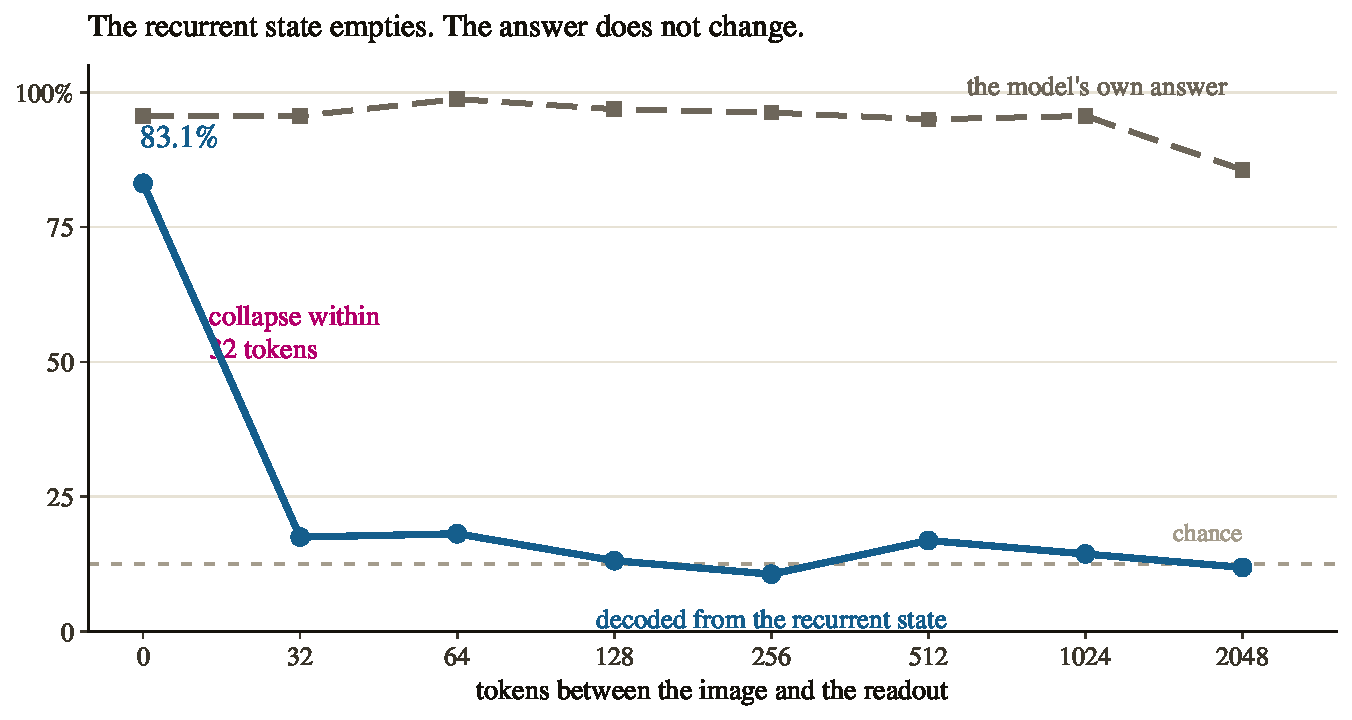
\includegraphics[width=0.86\linewidth]{../figures/pub/fig_cliff.pdf}
\caption{Probe accuracy against distance from the image. Object identity falls
from $83.1\%$ to $17.5\%$ between 0 and 32 tokens and stays near chance out to
2048. The three pre-image controls coincide at $12.5\%$. This is a step, not an
exponential: we deliberately do not quote a half-life, because fitting one to a
cliff produces a number ($469$ tokens) that describes nothing.}
\end{figure}

\subsection{Gist survives, particulars do not}

\begin{figure}[h]
\centering
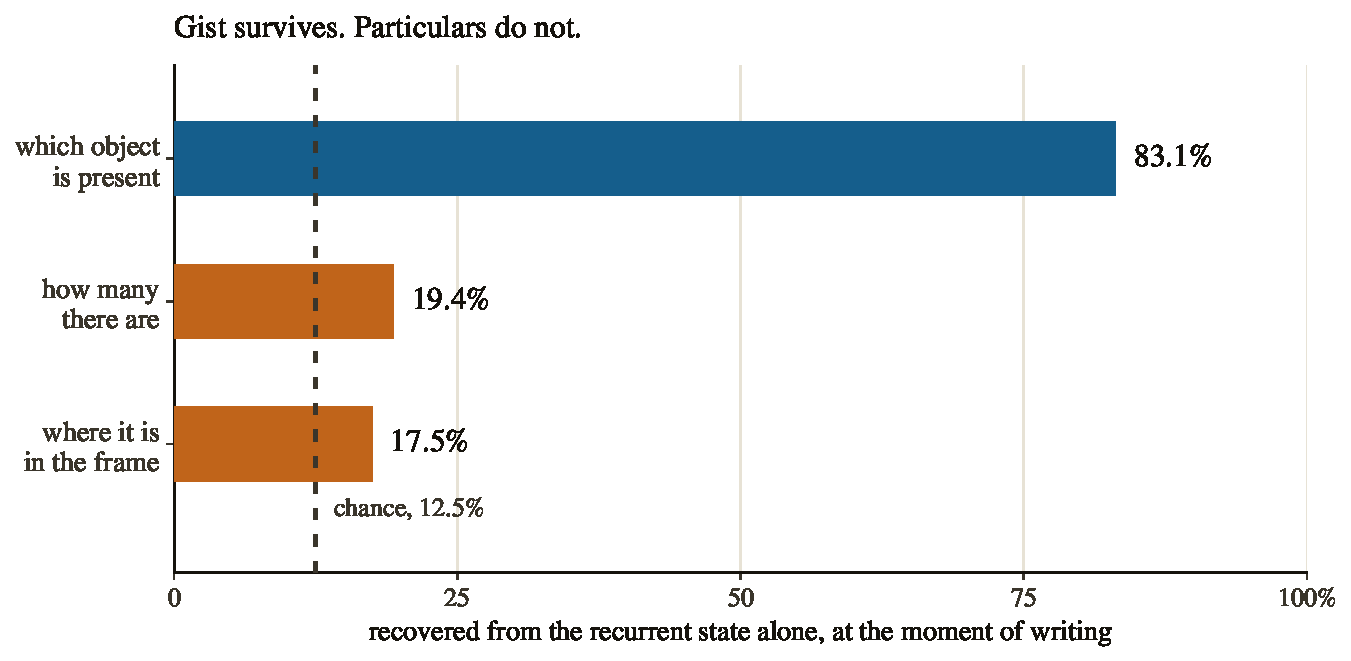
\includegraphics[width=0.92\linewidth]{../figures/pub/fig_gist.pdf}
\caption{At the moment of writing, the state is highly informative about which
object is present and barely informative about how many or where, from the
identical feature vectors.}
\end{figure}

\subsection{The answer comes from the 13 attention layers}

\begin{table}[h]
\centering\small
\begin{tabular}{@{}lrr@{}}
\toprule
\textbf{identity, $n=30$} & \textbf{follows own image} & \textbf{follows other image} \\
\midrule
no swap                          & 17 & 0 \\
all 81 recurrent states replaced & 19 & 0 \\
13 attention caches replaced     & 0  & 15 \\
both replaced                    & 0  & 14 \\
\bottomrule
\end{tabular}
\caption{The two lines cross. Every image is letterboxed to a common canvas so both runs emit
identical vision-token counts; zero pairs were dropped for length mismatch, and
the recurrent swap was verified to have taken effect in $90/90$ checks. That
``both'' matches ``attention'' establishes that attention alone determines the
answer.}
\end{table}

\begin{figure}[h]
\centering
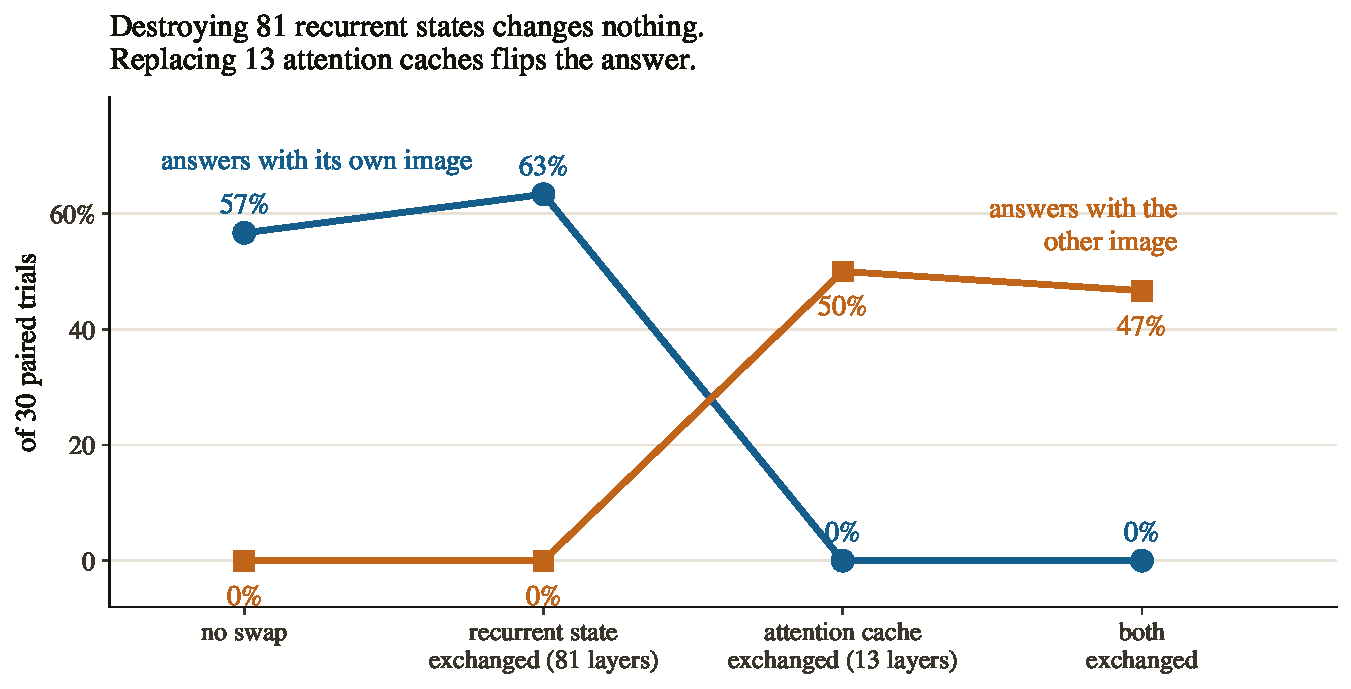
\includegraphics[width=0.92\linewidth]{../figures/pub/fig_splice.pdf}
\caption{The causal dissociation as a slope. Exchanging 81 recurrent states
leaves the answer with its own image; exchanging 13 attention caches moves it
entirely to the other image.}
\end{figure}

\section{Limitations}

\textbf{One model.} Every number here is Zamba2-VL-7B. The architecture class
is what makes the question meaningful, but a second hybrid VLM is needed before
any claim generalises to the class.
\textbf{Linear probes.} Absence of linear decodability is not absence of
information. The capacity control bounds this concern but does not eliminate
non-linear encodings.
\textbf{Splice baselines.} The model's own baseline on identity is $17/30$
under the letterboxed stimulus, so the flip is measured against a ceiling well
below one; count is uninformative for the splice because its baseline is at
noise.
\textbf{A methodological note recorded honestly.} Our first splice forced every
image to a square, which equalised token counts but distorted the images and
depressed identity accuracy from $17/30$ to $8/30$. The letterboxed design
fixes this. Both runs are in the repository.

\section{Conclusion}

An image enters this model's recurrent memory as a vivid impression of what
kind of thing it is, loses that impression within about thirty tokens, and none
of it matters: the answer was always being read from thirteen attention layers
out of eighty-one. The interesting object is not the forgetting. It is that a
memory can be measurably full and causally empty at the same time, and that in
the architectures now being deployed for efficiency, most of the memory is of
that kind.

\begin{thebibliography}{9}\small

\bibitem{jiang2026stateful}
J.~Jiang, A.~S. Deshmukh, K.~Chumachenko, K.~Sapra, Z.~Yu, G.~Liu, A.~Tao,
P.~Molchanov, J.~Kautz, and W.~Byeon.
\newblock Stateful Token Reduction for Long-Video Hybrid VLMs.
\newblock \emph{arXiv:2603.00198}, 2026.

\bibitem{abhinandan2026asktwice}
R.~H. Abhinandan, J.~Galeotti, D.~Ramanan, and G.~R. Gare.
\newblock Ask Twice, Look Twice: Prompt Echoing Resolves the Question-First
Paradox in Vision-Language Models.
\newblock \emph{arXiv:2607.15565}, 2026.

\bibitem{gupta2026modality}
A.~Gupta and Y.~Gandelsman.
\newblock Test-Time Training for Modality Order Consistency in Vision-Language
Models.
\newblock \emph{arXiv:2607.20351}, 2026.

\bibitem{osaka2026vab}
H.~Osaka, S.~Taniguchi, G.~Minegishi, K.~Yamashita, M.~Suzuki, and Y.~Matsuo.
\newblock Visual Access Boundaries in Vision-Language Model Reasoning.
\newblock \emph{arXiv:2607.12815}, 2026.

\bibitem{dao2024mamba2}
T.~Dao and A.~Gu.
\newblock Transformers are SSMs: Generalized Models and Efficient Algorithms
Through Structured State Space Duality.
\newblock \emph{ICML}, 2024.

\bibitem{lin2014coco}
T.-Y. Lin, M.~Maire, S.~Belongie, J.~Hays, P.~Perona, D.~Ramanan,
P.~Doll\'ar, and C.~L. Zitnick.
\newblock Microsoft COCO: Common Objects in Context.
\newblock \emph{ECCV}, 2014.

\bibitem{zamba2vl}
Zyphra.
\newblock Zamba2-VL-7B model card.
\newblock \url{https://huggingface.co/Zyphra/Zamba2-VL-7B}, 2026.
Apache-2.0.

\end{thebibliography}

\end{document}
